% !TEX TS-program = pdflatexmk
\documentclass[fyslu,english]{report}
\pagestyle{empty}

\usepackage[T1]{fontenc}
\usepackage{newtxmath,newtxtext}
\usepackage[english]{babel}
\usepackage{array, xcolor, lipsum, bibentry}
\usepackage[margin=2.3cm]{geometry}
%\usepackage{comment}
\usepackage{marginnote}
\usepackage{url}
\usepackage{longtable}
\usepackage{multirow, bigstrut}
\usepackage{hyperref}
\usepackage{colortbl}
\usepackage{graphicx,wrapfig,subfigure,transparent}
\graphicspath{
	{./}
	{./imm/}
	{./Fig/}
	}
\usepackage[yyyymmdd]{datetime}
\usepackage{pdfpages}
\renewcommand{\dateseparator}{}
%\usepackage[
%	backend=biber,
%%	bibstyle=verbose,
%%	bibstyle=reading,
%%	bibstyle=authoryear,
%%	bibstyle=authortitle,
%	style=alphabetic,
%%	bibstyle=debug,
%	sorting=anyvt,
%	maxnames=3,
%	firstinits=true
%	]{biblatex} 
%%\DeclareNameAlias{sortname}{first-last}
%\bibliography{
%	%~/BibTex/SoNnIG,
%	~/BibTex/Varie,
%}
\usepackage{siunitx}
\usepackage{lastpage}
\usepackage{advdate}

\newcommand*{\email}[1]{\href{mailto:#1}{\nolinkurl{#1}} } 

%\usepackage{acronym}
%\input{./acronym.tex}

\usepackage{fancyhdr}
\pagestyle{fancy}
\fancyhf{}
\lhead{\includegraphics[height=0.5cm]{/Users/frame/Pictures/Logos/dnplusonnig-sonnig_logo-14963c6d0485/sonnig_logo_without_text.pdf}}
\rhead{CERBERUS DATA SHEET v.\today}
\lfoot{SOurce-based NeutroN Irradiation Group  -  sonnig@nuclear.lu.se}
\rfoot{\thepage\ of \pageref{LastPage}}
%\renewcommand{\headrulewidth}{2pt}
\renewcommand{\footrulewidth}{.5pt}

\begin{document}
\begin{center} 
{\Large DATA SHEET} \vspace{0.5cm}

\vspace{3cm}
{\Huge \textbf{ CERBERUS } }
\\ \vspace{1cm}{\Large (1 to 3 analog fully differential Fan-Out)}
%\\ \vspace{1cm}{\AdvanceDate[-1]\today} 
\\ \vspace{1cm} {F. Messi}
\\ \vspace{1.5cm}
{\transparent{1}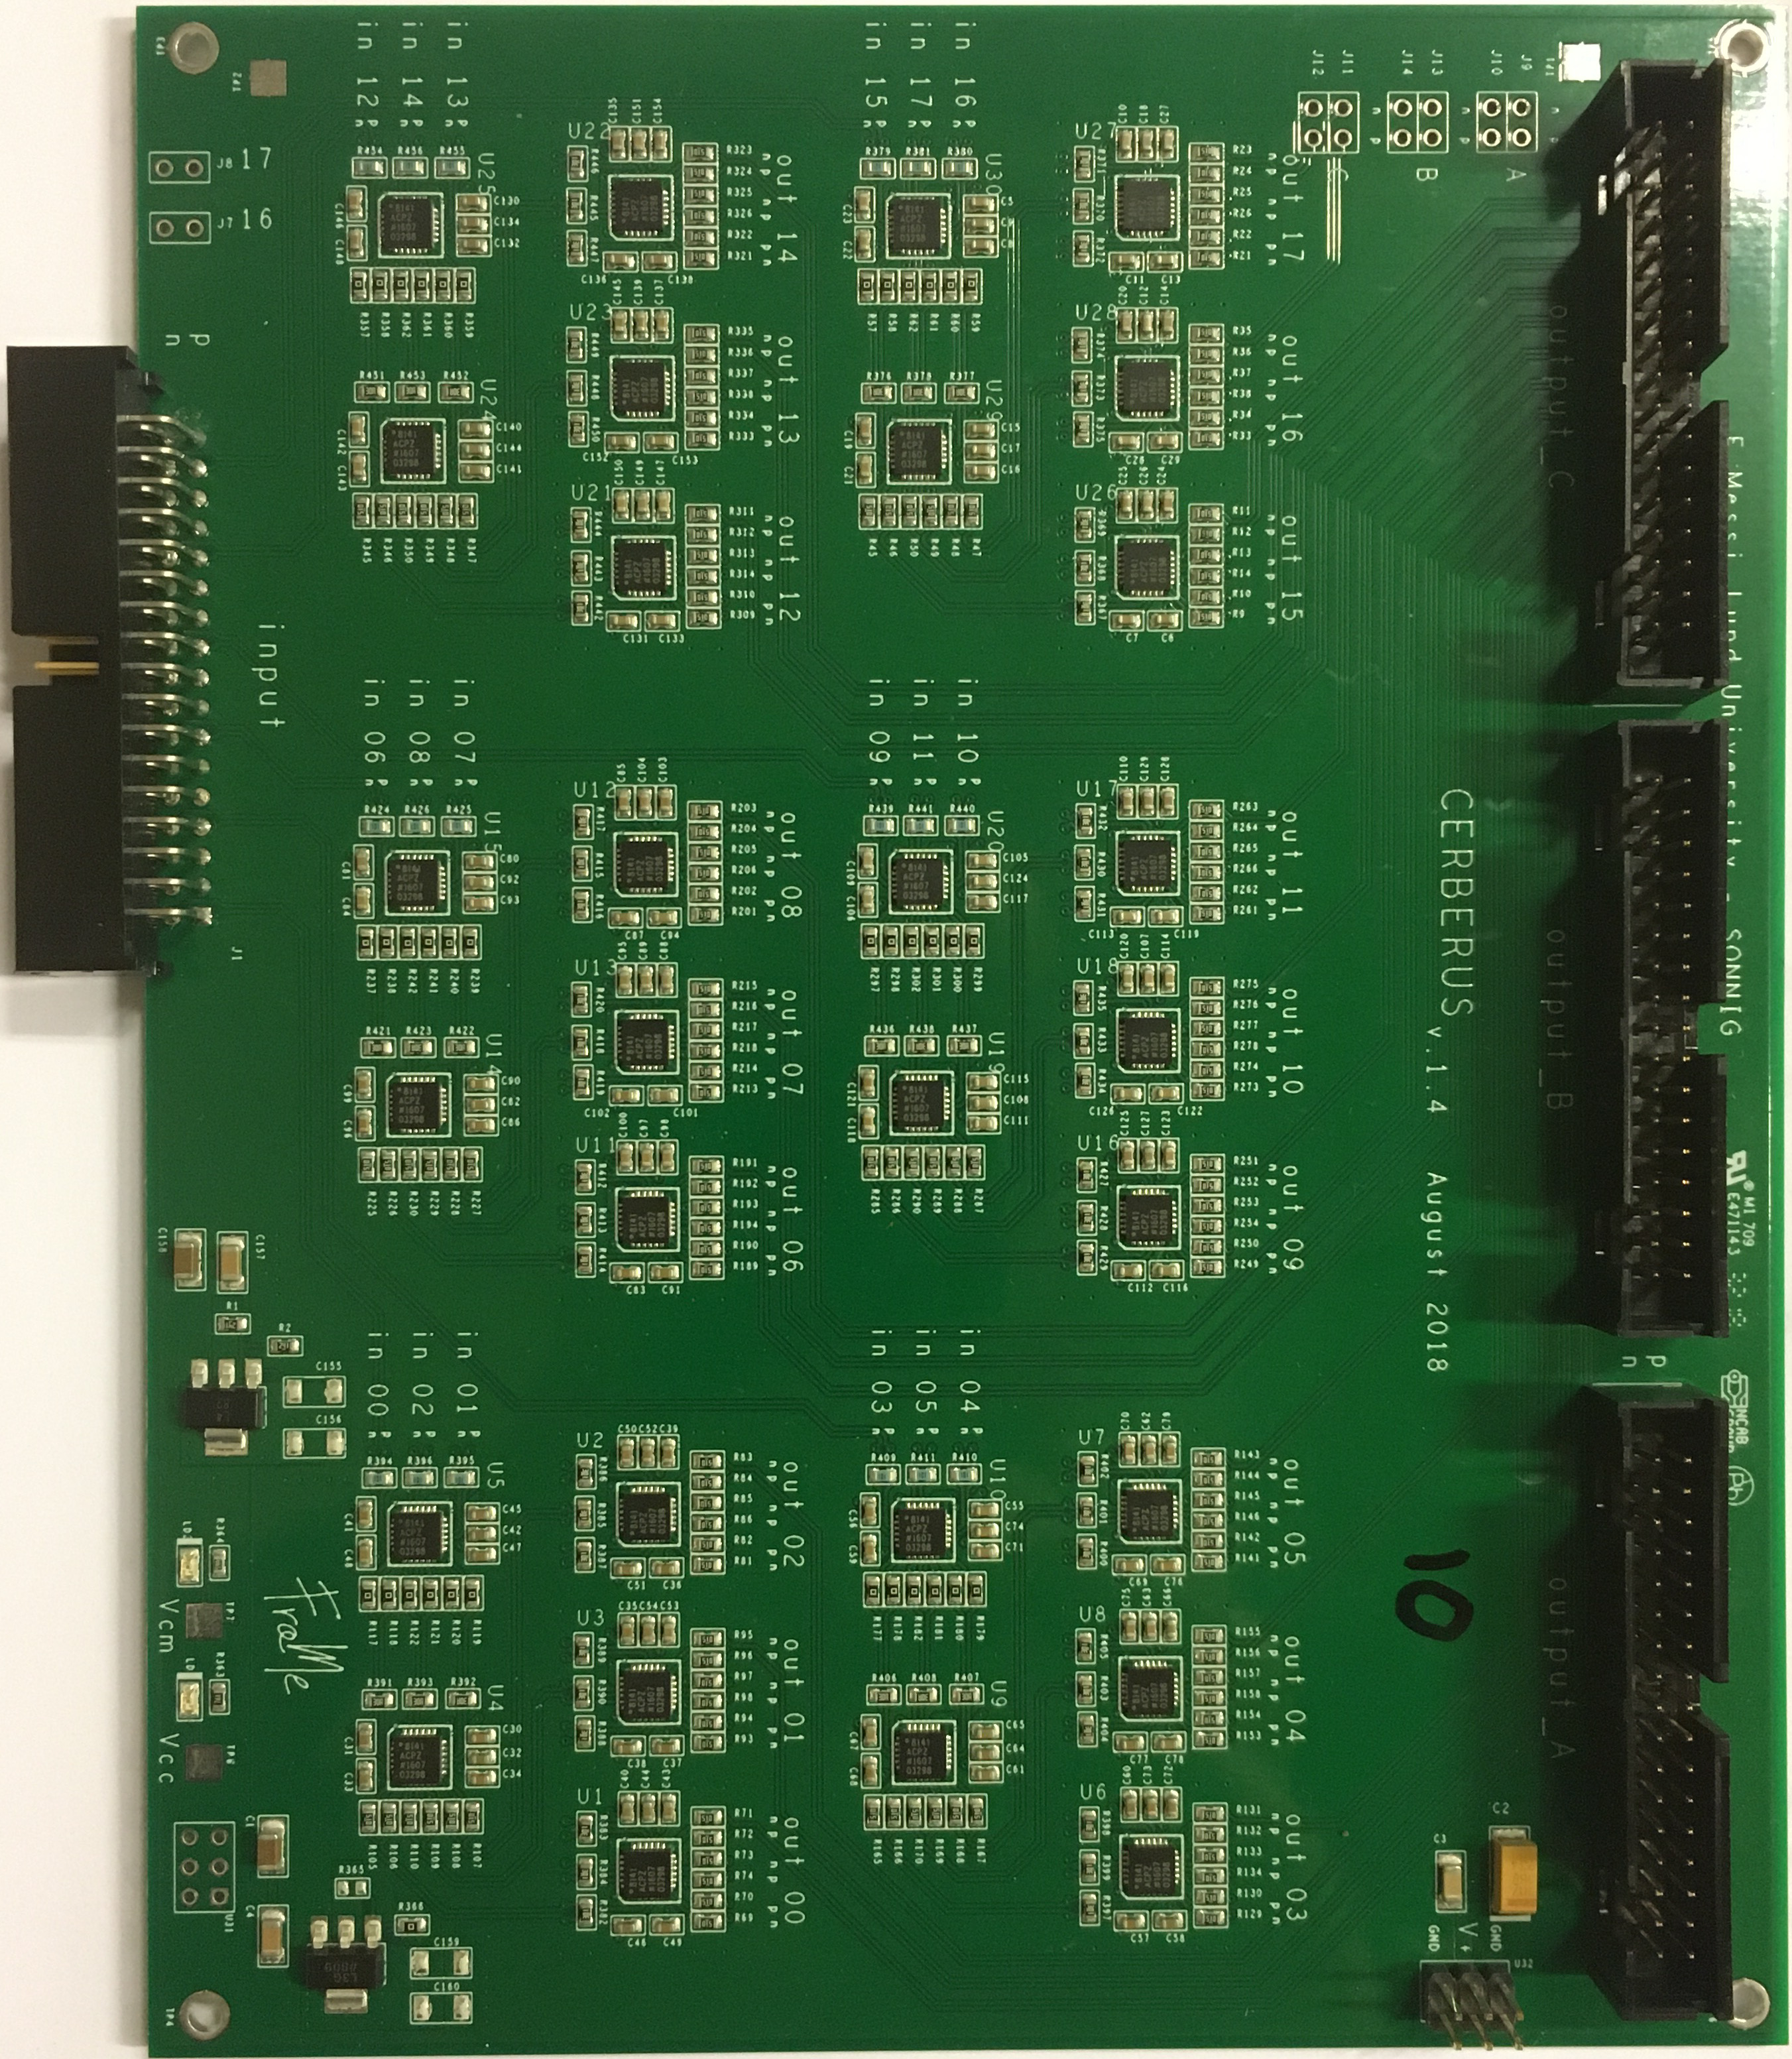
\includegraphics[width=0.6\textwidth]{IMG_9270}}
\end{center} 

%\newpage
%\tableofcontents

\newpage
\section{Description}
The CERBERUS board is a fully differential analog Fan-Out with a ratio $1$ to $3$. 
While the board has been designed to obtain three identical copies of the output signal from the \emph{MA\_PRE}, it can accept any differential analog signal in the dynamic range. 

The board is based on the \emph{AD8141 Triple Differential Drivers.}  

The power on the board is regulated and an input voltage of $+6\,\si\V$ is recommended. \\

The board has a total of $18$ input channels, $16$ on the input connetor plus two on dedicated pins. 
The outputs of the board are labled $A$, $B$ and $C$.

\begin{figure}[htbp]
\begin{center}
%	\subfigure[\footnotesize  \label{labelA}]{\includegraphics[width=0.4\textwidth]{cs}}\qquad
%	\subfigure[\footnotesize  \label{labelB}]{\includegraphics[width=0.4\textwidth]{cs}} 
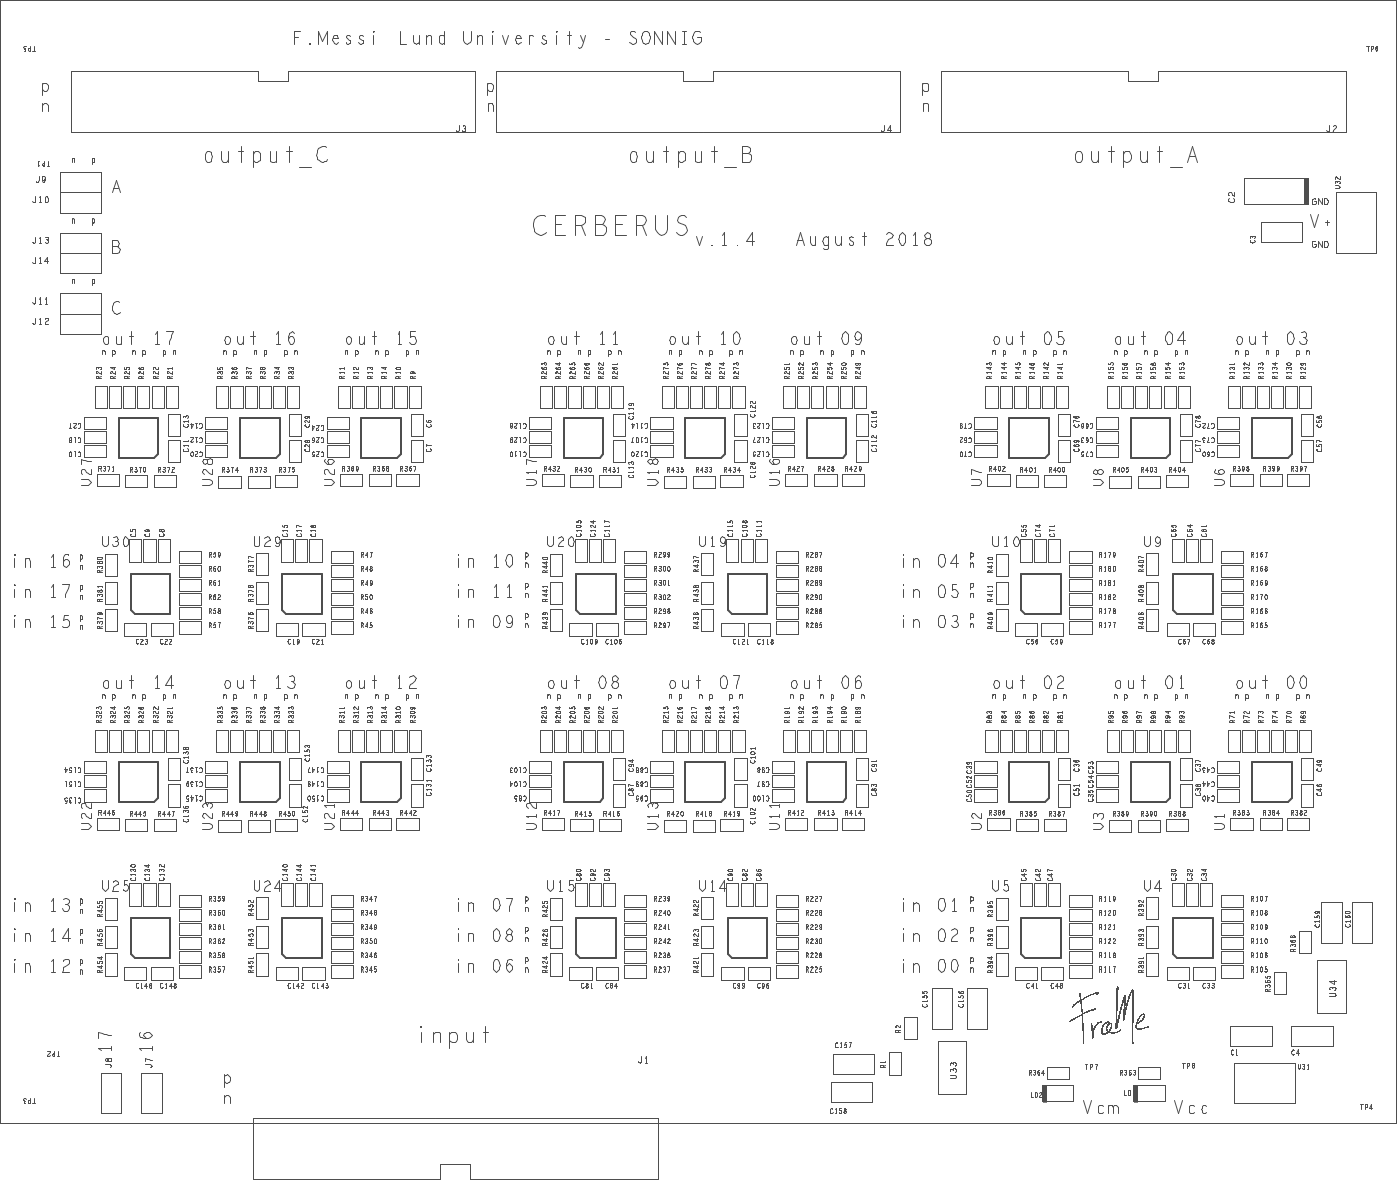
\includegraphics[width=0.9\textwidth]{Cerberus_v1-4_SLKTOP.png}%CerberusConnectors}
\caption{Connectors on the CERBERUS board.}
\label{fig.connectors}
\end{center}
\end{figure}

\section{Power connection}
To board is powered via \emph{connector U32}; accepted voltage is $+6\,\si\V$ on the two central pins on the connector; the side four pins are GND. 
Current consumption on the board is $\approx 1.6\,\si\A$.

\newpage

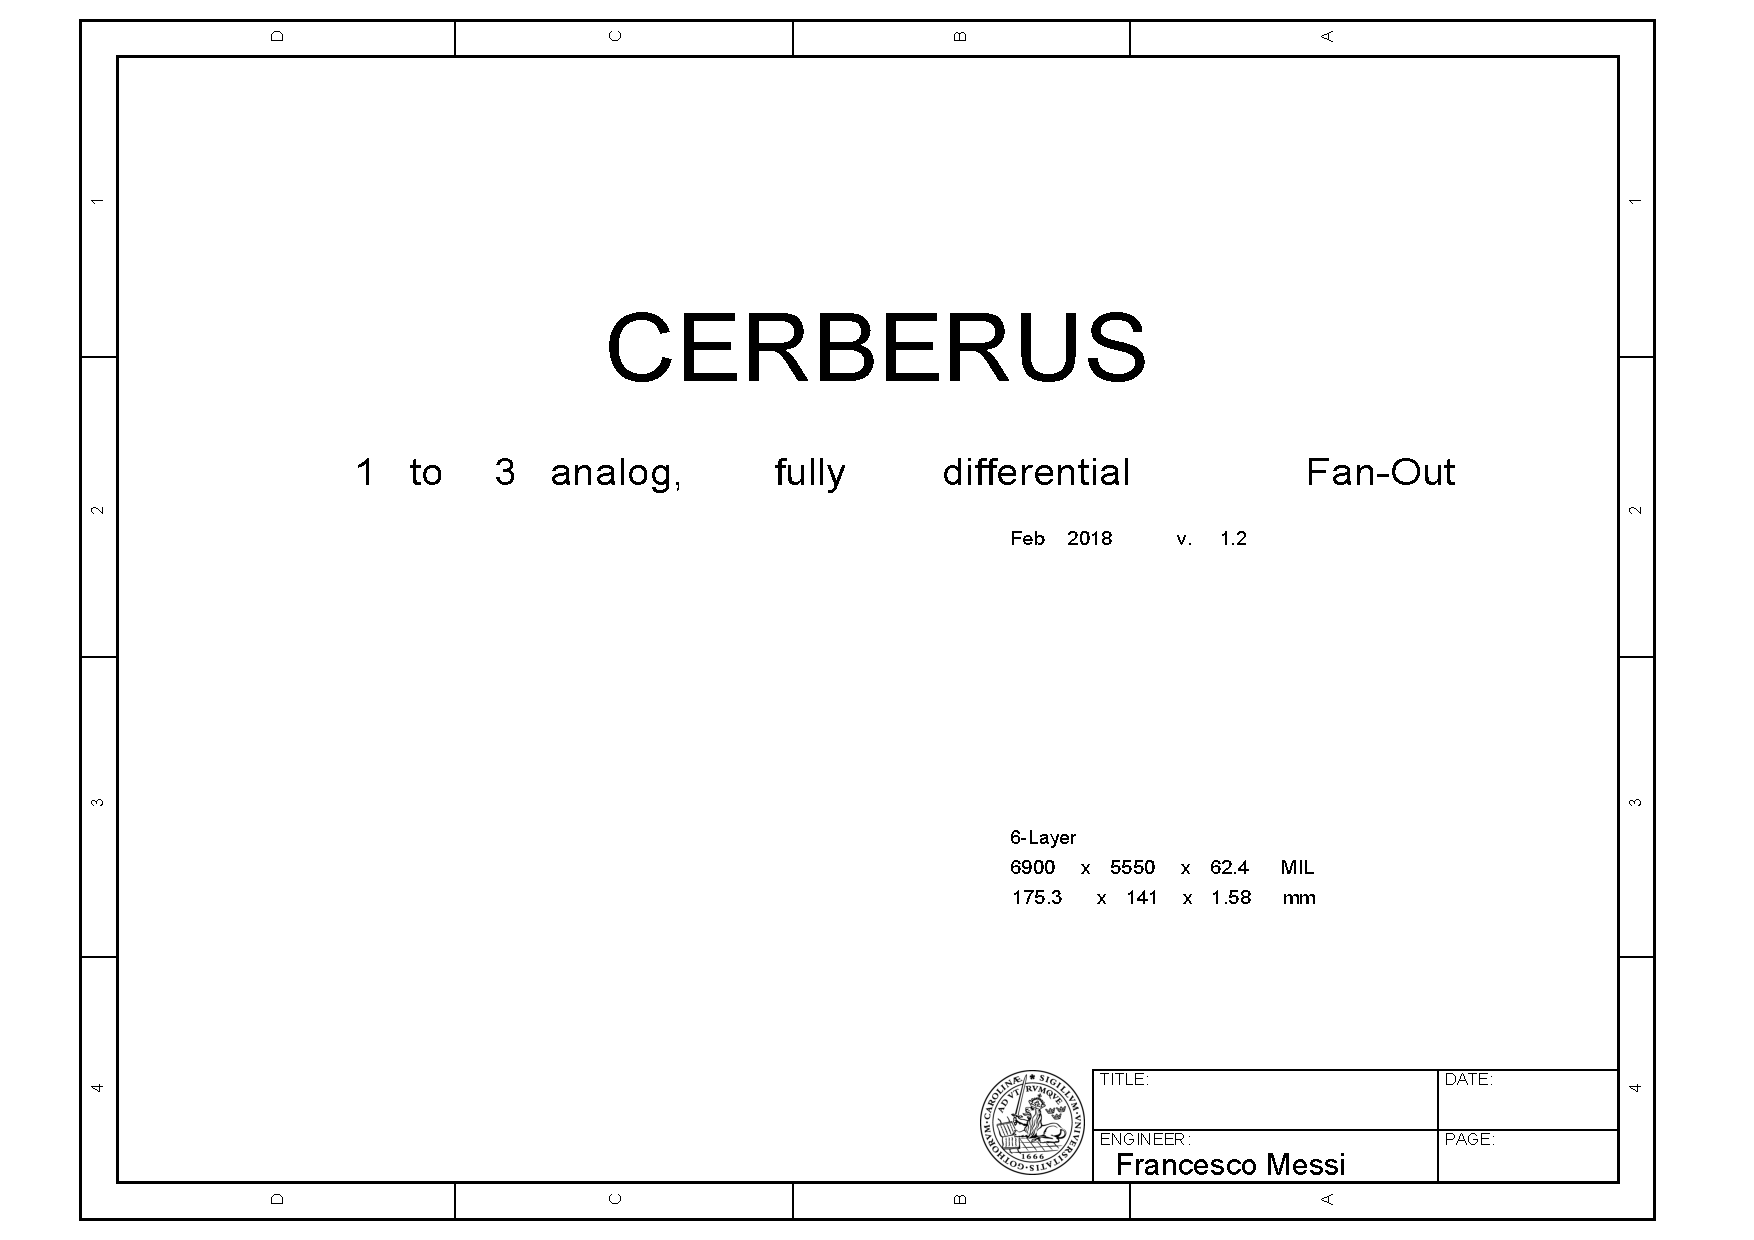
\includepdf[pages=1-3]{Fig/Cerberus_v1-2.pdf} \includepdf[pages=9-10]{Fig/Cerberus_v1-2.pdf} %schematics
\includepdf[pages=11-16]{Fig/Cerberus_v1-2.pdf} % layers

\end{document}


%=============================

\begin{figure}[htbp]
\begin{center}
%	\subfigure[\footnotesize  \label{labelA}]{\includegraphics[width=0.4\textwidth]{cs}}\qquad
%	\subfigure[\footnotesize  \label{labelB}]{\includegraphics[width=0.4\textwidth]{cs}} 
\includegraphics[width=0.6\textwidth]{sampling}
\caption{default}
\label{fig.sampling}
\end{center}
\end{figure}

%=============================

\begin {table}[h]
\begin{center}
\begin{tabular}{c | c | c | m{5cm}| c |  c }
\bf{\large Name} & \bf{\large Surname} & \bf{\large email} &  \bf{{\large \center Essay title}} & \bf{\large Referee 1} & \bf{\large Referee 2} \\ \hline \hline \bigstrut 

\end{tabular}
%\caption{default}
\label{tab.Titles}
\end{center}
\end{table}
